% =====================================================================
%  BAB 6 — PENGUJIAN DAN ANALISIS
% =====================================================================

\chapter{Pengujian dan Analisis}

\section{Prosedur Pengujian}
\label{sec:6.1}

[Jelaskan prosedur pengujian yang dilaksanakan, mengacu pada rancangan pengujian di
Seksyen~\ref{sec:4.6}. Uraikan urutan langkah, konfigurasi yang digunakan, dan cara
hasil dikumpulkan.]

% Contoh: diagram alur pengujian
\begin{figure}[H]
  \centering
  \begin{tikzpicture}[node distance=0.9cm]
    \node[term]     (mulai)  {Mulai};
    \node[io]       (setup)  [below=of mulai]  {Inisialisasi lingkungan};
    \node[proc]     (data)   [below=of setup]  {Muat data uji};
    \node[proc]     (jalankan)[below=of data]  {Jalankan skenario};
    \node[io]       (kumpul) [below=of jalankan]{Kumpulkan metrik};
    \node[dec]      (ulang)  [below=of kumpul] {Semua skenario\\selesai?};
    \node[proc]     (analisis)[below=of ulang] {Analisis \& visualisasi};
    \node[term]     (selesai)[below=of analisis]{Selesai};
    \node[proc]     (iterasi)[right=2cm of ulang]{Skenario\\berikutnya};

    \draw[arr] (mulai)    -- (setup);
    \draw[arr] (setup)    -- (data);
    \draw[arr] (data)     -- (jalankan);
    \draw[arr] (jalankan) -- (kumpul);
    \draw[arr] (kumpul)   -- (ulang);
    \draw[arr] (ulang)    -- node[flbl,right]{Ya} (analisis);
    \draw[arr] (ulang)    -- node[flbl,above]{Tidak} (iterasi);
    \draw[arr] (iterasi)  |- (data);
    \draw[arr] (analisis) -- (selesai);
  \end{tikzpicture}
  \caption{Alur prosedur pengujian}
  \label{fig:6.alur}
\end{figure}

% ── 6.2 Hasil Pengujian Utama ────────────────────────────────────────
\section{Hasil Pengujian [Aspek Utama 1]}
\label{sec:6.2}

[Sajikan hasil pengujian skenario pertama. Gunakan tabel untuk angka, grafik untuk tren.
Deskripsikan temuan secara faktual sebelum memberikan interpretasi.]

\begin{table}[H]
  \centering
  \caption{Hasil [Aspek Utama 1] pada berbagai konfigurasi}
  \label{tab:6.hasil1}
  \begin{tabular}{lrrrr}
    \toprule
    \textbf{Konfigurasi} & \textbf{Presisi} & \textbf{Recall} & \textbf{F1} & \textbf{Latensi (ms)} \\
    \midrule
    {[Konfigurasi A]} & [0,XX] & [0,XX] & [0,XX] & [X,XX] \\
    {[Konfigurasi B]} & [0,XX] & [0,XX] & [0,XX] & [X,XX] \\
    {[Konfigurasi C]} & [0,XX] & [0,XX] & [0,XX] & [X,XX] \\
    \textbf{Sistem ini} & \textbf{[0,XX]} & \textbf{[0,XX]} & \textbf{[0,XX]} & \textbf{[X,XX]} \\
    \bottomrule
  \end{tabular}
\end{table}

% Contoh grafik pgfplots (bar chart)
\begin{figure}[H]
  \centering
  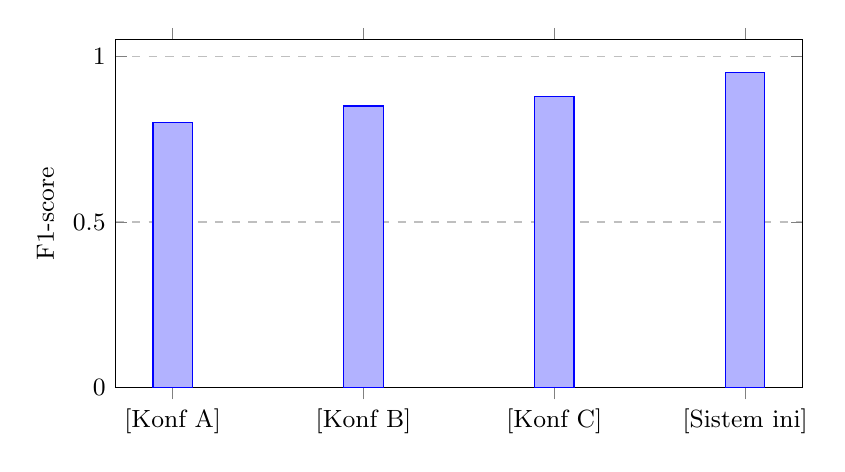
\begin{tikzpicture}
    \begin{axis}[
      ybar, bar width=0.5cm,
      width=0.85\textwidth, height=6cm,
      ylabel={F1-score},
      xtick=data,
      xticklabels={[Konf A],[Konf B],[Konf C],[Sistem ini]},
      ymin=0, ymax=1.05,
      ymajorgrids=true, grid style=dashed,
      legend pos=north west,
      tick label style={font=\small},
      label style={font=\small},
    ]
      \addplot coordinates {(0,0.80) (1,0.85) (2,0.88) (3,0.95)};
    \end{axis}
  \end{tikzpicture}
  \caption{Perbandingan F1-score antar konfigurasi}
  \label{fig:6.f1}
\end{figure}

[Analisis: mengapa konfigurasi terbaik mengungguli yang lain? Faktor apa yang berkontribusi?]

% ── 6.3 Hasil Pengujian Aspek 2 ──────────────────────────────────────
\section{Hasil Pengujian [Aspek 2]}
\label{sec:6.3}

[Sajikan hasil skenario kedua. Contoh: pengujian skalabilitas, latensi, throughput, dsb.]

% Contoh: grafik garis (latensi vs beban)
\begin{figure}[H]
  \centering
  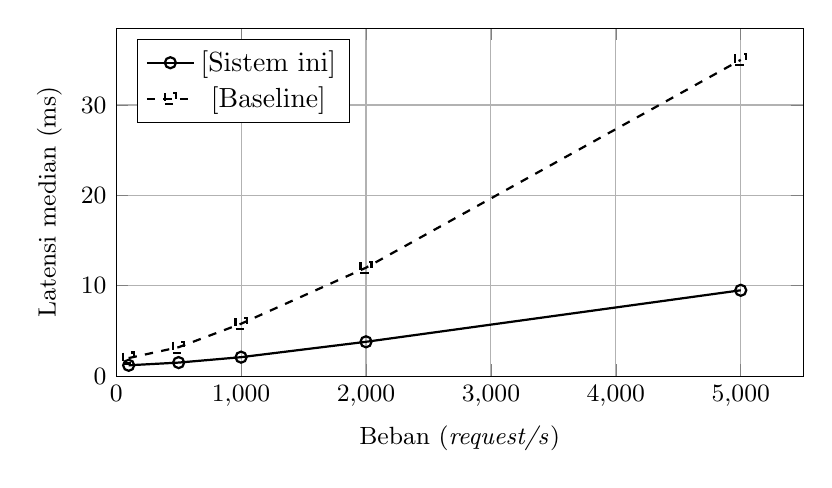
\begin{tikzpicture}
    \begin{axis}[
      width=0.85\textwidth, height=6cm,
      xlabel={Beban (\emph{request/s})},
      ylabel={Latensi median (ms)},
      xmin=0, ymin=0,
      grid=both, grid style={line width=.2pt, draw=gray!30},
      major grid style={line width=.4pt, draw=gray!60},
      legend pos=north west,
      tick label style={font=\small},
      label style={font=\small},
    ]
      \addplot[mark=o, thick] coordinates {
        (100,1.2) (500,1.5) (1000,2.1) (2000,3.8) (5000,9.5)
      };
      \addlegendentry{[Sistem ini]}
      \addplot[mark=square, thick, dashed] coordinates {
        (100,2.0) (500,3.2) (1000,5.8) (2000,12.0) (5000,35.0)
      };
      \addlegendentry{[Baseline]}
    \end{axis}
  \end{tikzpicture}
  \caption{Latensi median terhadap beban}
  \label{fig:6.latensi}
\end{figure}

% ── 6.4 Analisis Ablasi ──────────────────────────────────────────────
\section{Analisis Ablasi}
\label{sec:6.4}

[Tunjukkan kontribusi masing-masing komponen/fitur dengan mematikannya satu per satu
dan mengukur dampak performa. Ini adalah bagian yang membuktikan bahwa setiap pilihan
desain berkontribusi nyata.]

\begin{table}[H]
  \centering
  \caption{Hasil ablasi komponen sistem}
  \label{tab:6.ablasi}
  \begin{tabular}{lcccr}
    \toprule
    \textbf{Variasi} & \textbf{[Komponen A]} & \textbf{[Komponen B]} & \textbf{[Komponen C]}
                     & \textbf{F1} \\
    \midrule
    Sistem penuh     & \checkmark & \checkmark & \checkmark & [0,XX] \\
    Tanpa [Komp C]   & \checkmark & \checkmark & --         & [0,XX] \\
    Tanpa [Komp B]   & \checkmark & --         & \checkmark & [0,XX] \\
    Tanpa [Komp A]   & --         & \checkmark & \checkmark & [0,XX] \\
    \emph{Baseline}  & --         & --         & --         & [0,XX] \\
    \bottomrule
  \end{tabular}
\end{table}

[Diskusi: komponen mana yang paling berkontribusi dan mengapa.]

% ── 6.5 Perbandingan dengan Penelitian Terdahulu ─────────────────────
\section{Perbandingan dengan Penelitian Terdahulu}
\label{sec:6.5}

[Bandingkan hasil sistem Anda dengan hasil yang dilaporkan pada penelitian terdahulu
(Bab~2). Perhatikan: perbandingan yang adil mensyaratkan dataset dan skenario yang sama
atau setara. Jelaskan keterbatasan perbandingan jika ada.]

\begin{table}[H]
  \centering
  \caption{Perbandingan dengan penelitian terdahulu}
  \label{tab:6.komparasi}
  \begin{tabular}{lp{2.8cm}rrr}
    \toprule
    \textbf{Penelitian} & \textbf{Dataset} & \textbf{F1} & \textbf{Latensi (ms)}
                        & \textbf{[Metrik lain]} \\
    \midrule
    {[Peneliti A, Tahun]} & [Nama dataset] & [0,XX] & [X,X] & [X] \\
    {[Peneliti B, Tahun]} & [Nama dataset] & [0,XX] & [X,X] & [X] \\
    \textbf{Penelitian ini} & [Nama dataset] & \textbf{[0,XX]} & \textbf{[X,X]} & \textbf{[X]} \\
    \bottomrule
  \end{tabular}
\end{table}

% ── 6.6 Diskusi ──────────────────────────────────────────────────────
\section{Diskusi}
\label{sec:6.6}

\subsection{Keterbatasan Sistem}
\label{sec:6.6.1}

[Bahas secara jujur keterbatasan sistem yang dibangun: kondisi di mana performa menurun,
asumsi yang mungkin tidak berlaku di lingkungan produksi nyata, dsb.]

\subsection{Ancaman terhadap Validitas}
\label{sec:6.6.2}

[Identifikasi ancaman terhadap validitas hasil eksperimen: \emph{internal validity}
(apakah perubahan memang disebabkan sistem Anda?), \emph{external validity} (apakah
hasil dapat digeneralisasi?), dan \emph{construct validity} (apakah metrik yang dipilih
benar-benar mengukur yang dimaksud?).]
